\section{Tasks \#1. Freelook and spectral files.}

\subsection{Colorchecker 121 ms}

\subsubsection{Gray scale preview}
Wavelength 429 nm was selected for the gray scale preview. The preview of the colorchecker and the spectra are shown in Figure \ref{fig:cc-gray}.

\begin{figure}[H] %
  \centering
  \subfloat[On blue colored area]{%
    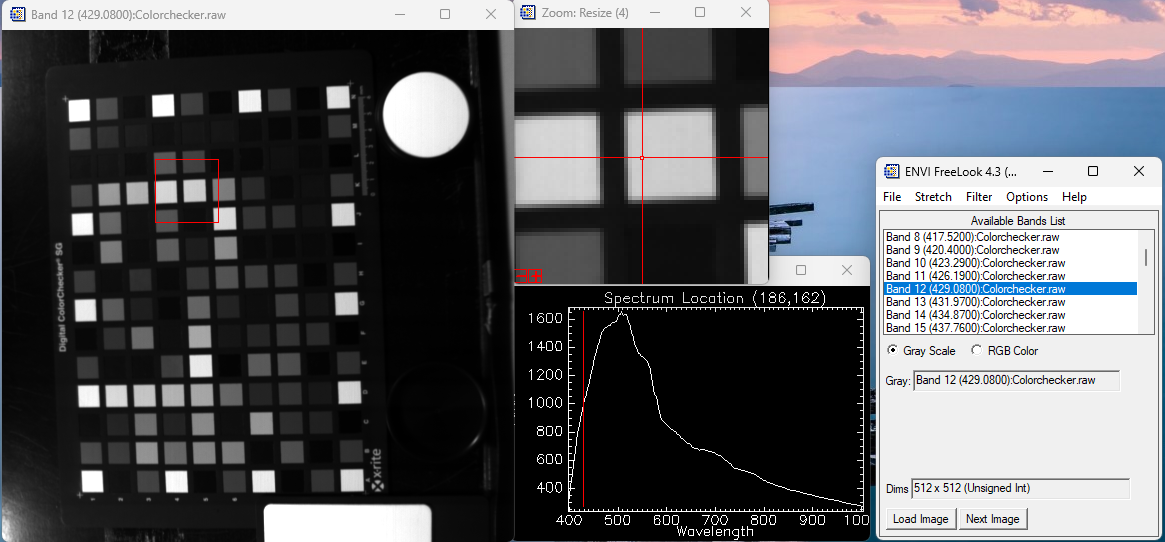
\includegraphics[width=0.45\textwidth]{
      figs/colorchecker_freelook_gray_blue.png
    }
  }
  \hspace{0.1cm}
  \subfloat[On pink colored area]{%
    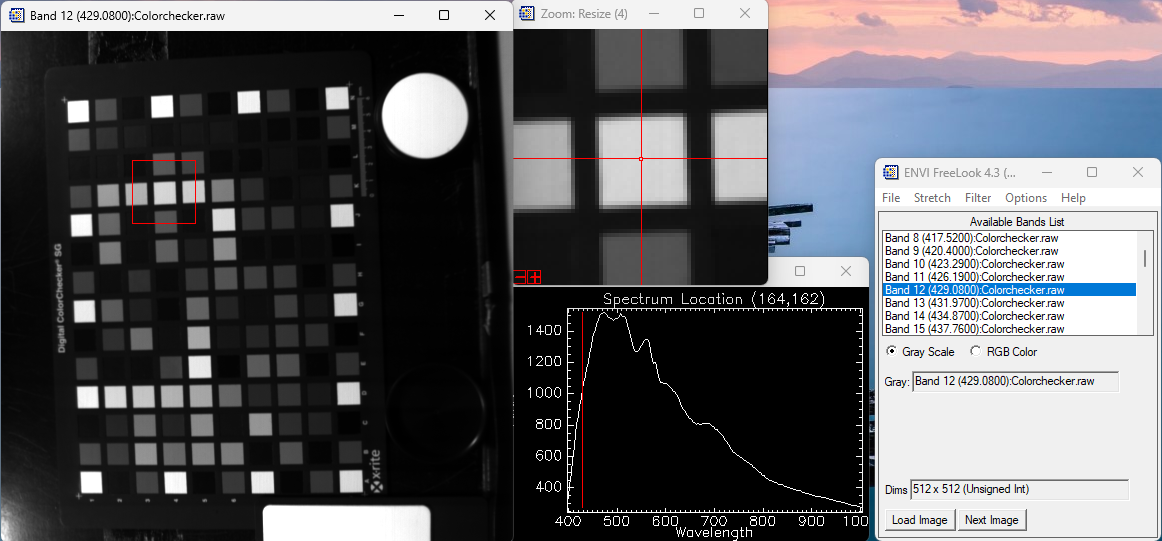
\includegraphics[width=0.45\textwidth]{
      figs/colorchecker_freelook_gray_pink.png
    }
  }
  \caption[]{Gray preview of colorchecker and spectra }
  \label{fig:cc-gray}
\end{figure}

\subsubsection{RGB preview}
Wavelengths 429 nm, 533 nm, and 631 nm were selected for the RGB preview. The preview of the colorchecker and the spectra are shown in Figure \ref{fig:cc-rgb}. White correction was not applied to the spectra. Thus, the color of these images is "natural".

\begin{figure}[H] %
  \centering
  \subfloat[On blue colored area]{%
    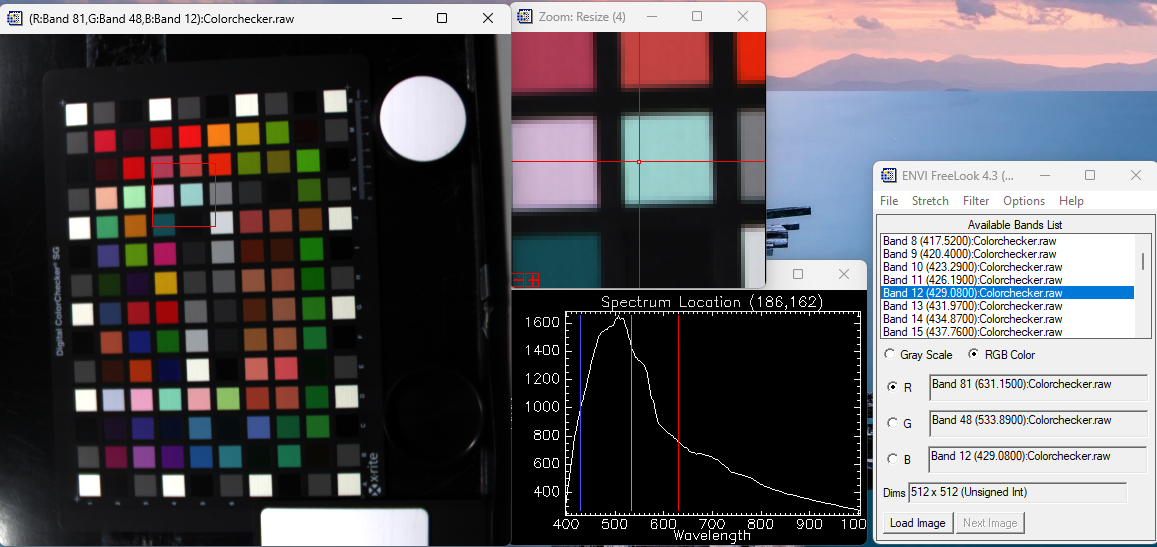
\includegraphics[width=0.45\textwidth]{
      figs/colorchecker_freelook_rgb_blue.png
    }
  }
  \hspace{0.1cm}
  \subfloat[On pink colored area]{%
    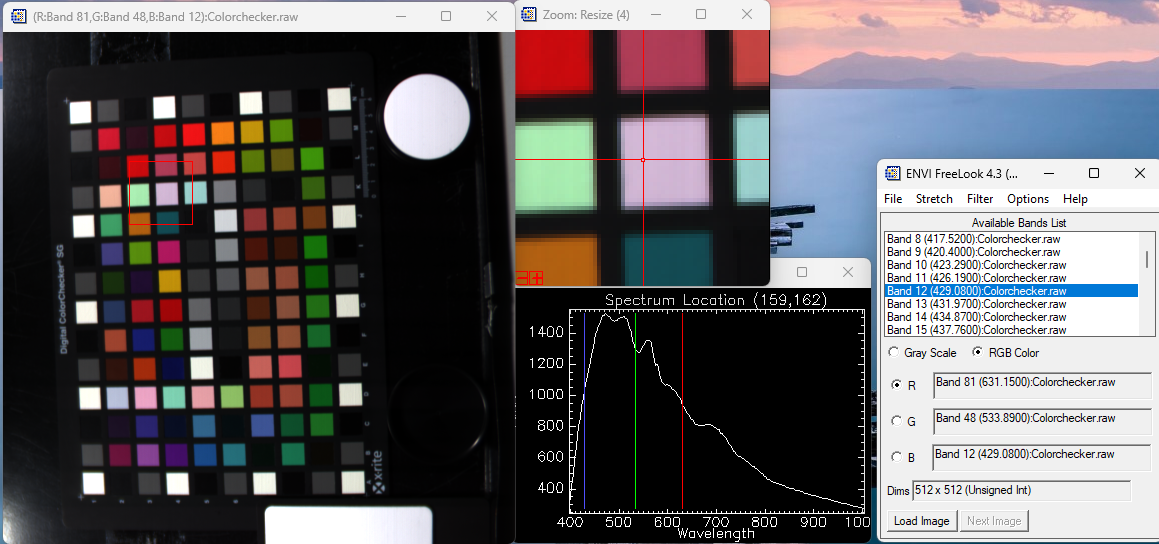
\includegraphics[width=0.45\textwidth]{
      figs/colorchecker_freelook_rgb_pink.png
    }
  }
  \caption[]{RGB preview of colorchecker and spectra }
  \label{fig:cc-rgb}
\end{figure}

\subsection{Leaves (Specim IQ)}

The spectral images of live and plastic leaves are shown in Figure \ref{fig:leaves}.

Wavelength 750 nm was selected for the gray scale preview.
Wavelengths 429 nm, 533 nm, and 750 nm were selected for the RGB preview.

At 750 nm, plastic leaves and live leaves have different reflectance. The plastic leaves have higher reflectance than the live leaves. This is because the plastic leaves are more reflective in the near-infrared region.

\begin{figure}[H] %
  \centering
  \subfloat[Gray scale preview]{%
    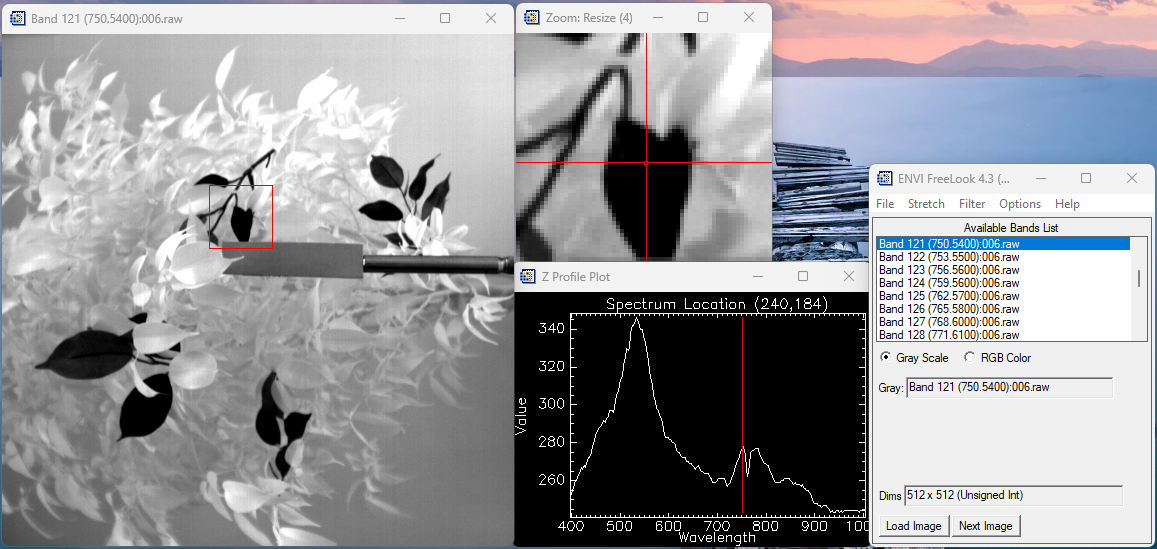
\includegraphics[width=0.45\textwidth]{
      figs/leaves_gray.png
    }
  }
  \hspace{0.1cm}
  \subfloat[RGB scale preview]{%
  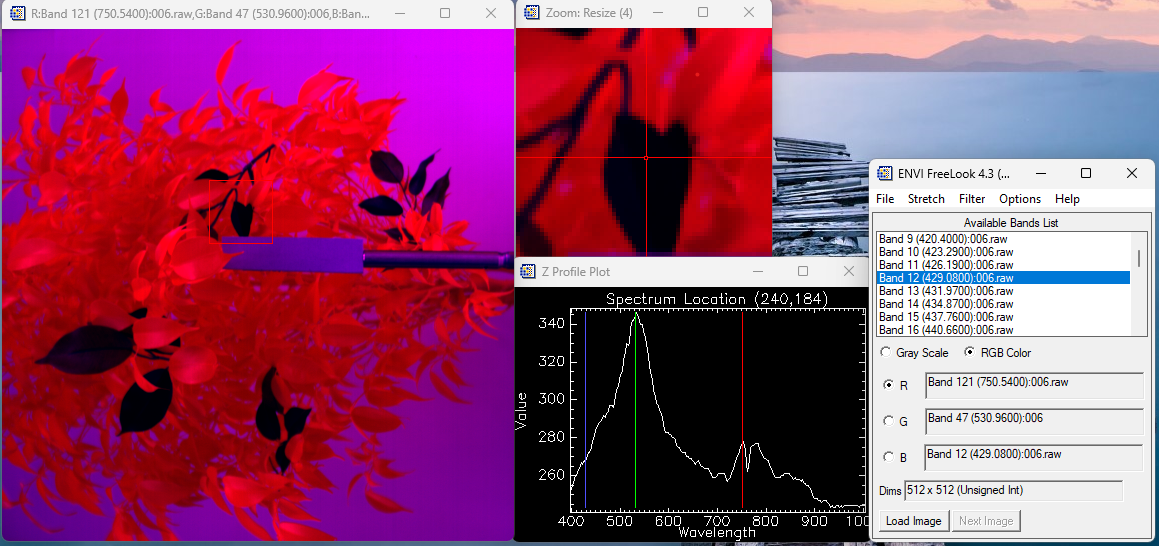
\includegraphics[width=0.45\textwidth]{figs/leaves_rgb.png}}
  \caption[]{Spectral image of live and plastic leaves }
  \label{fig:leaves}
\end{figure}

\subsection{Infrared (by sarita.keski-saari@uef.fi)}

The figure \ref{fig:painting} shows an RGB preview of a painting. This image was captured with infrared wavelength range. Three wavelength, 2399 nm, 1496 nm, and 1275 nm were selected to construct the RGB preview. This is why the preview does not look "natural".

The original RGB picuture of this painting is shown in Figure \ref{fig:painting-org}.
In Figure \ref{fig:painting}, some obstacles like stamp of coffee cup are visible. Using infrared spectral image, we can observe hidden features, not only paintings in visible range.

\begin{figure}[H]
  \centering
  \caption{Infrared spectral image of a painting}
  \label{fig:painting}
  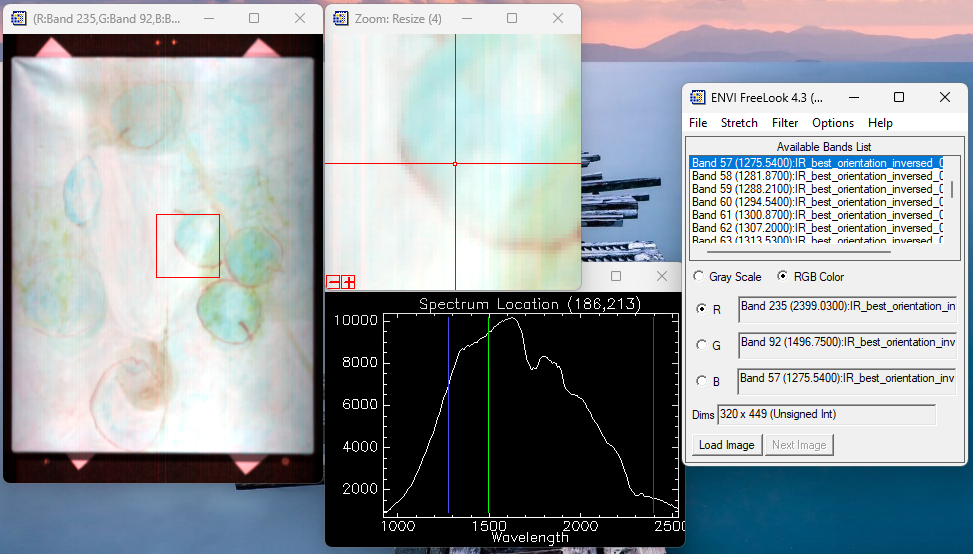
\includegraphics[width=0.5\textwidth]{./figs/painting.png}
\end{figure}

\begin{figure}[H]
  \centering
  \caption{Original RGB view of the paingin}
  \label{fig:painting-org}
  \includegraphics[width=0.5\textwidth]{./figs/painting_visible.png }
\end{figure}

\subsection{124 (rock painting)}

The rock painting has inked areas and other areas. The spectra of inked areas and other areas are shown in Figure \ref{fig:rock-painting}.

Right-side of Figure \ref{fig:rock-painting-ink1} and Figure \ref{fig:rock-painting-ink2} shows the spectra of inked areas. These two spectras have similar distribution compared to the spectra of rock surface shown in Figure \ref{fig:rock-painting-other}. Thus, we can say that painted areas have same ink.

\begin{figure}[H]
  \centering
  \subfloat[Spectra of inked area]{
    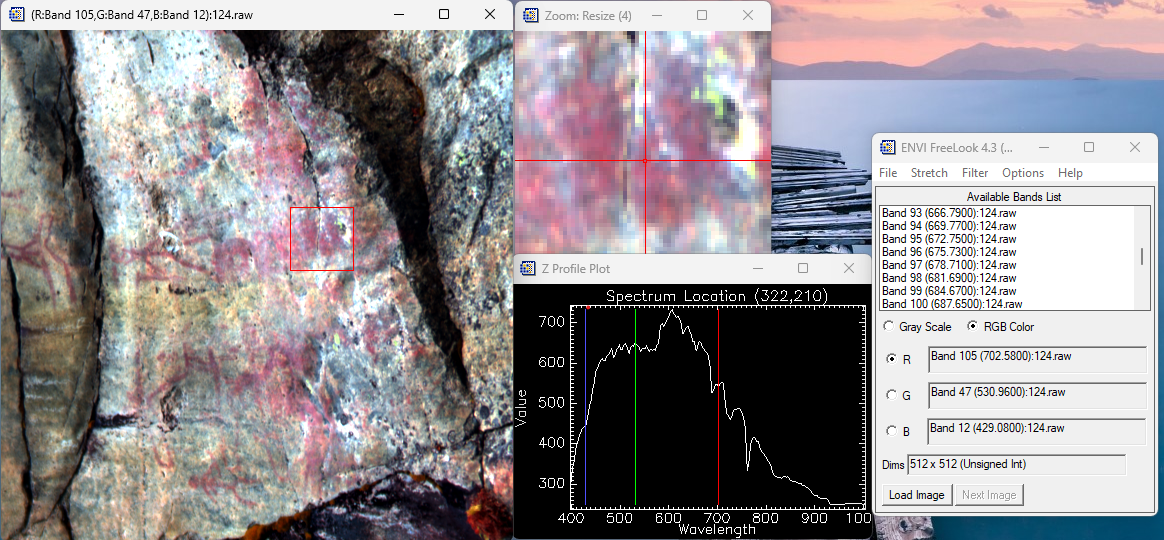
\includegraphics[width=0.45\textwidth]{figs/rock_painting_ink1.png}
    \label{fig:rock-painting-ink1}
  }
  \hspace{0.1cm}
  \subfloat[Another inked area]{
    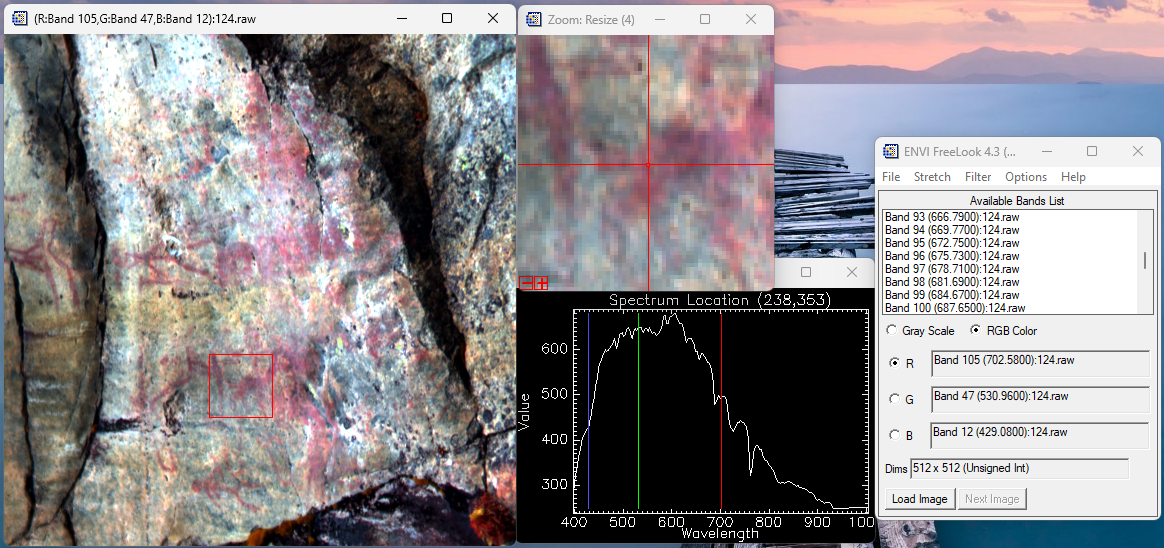
\includegraphics[width=0.45\textwidth]{figs/rock_painting_ink2.png}
    \label{fig:rock-painting-ink2}
  }
  \vspace{0.1cm}
  \subfloat[Spectra of rock surface]{
    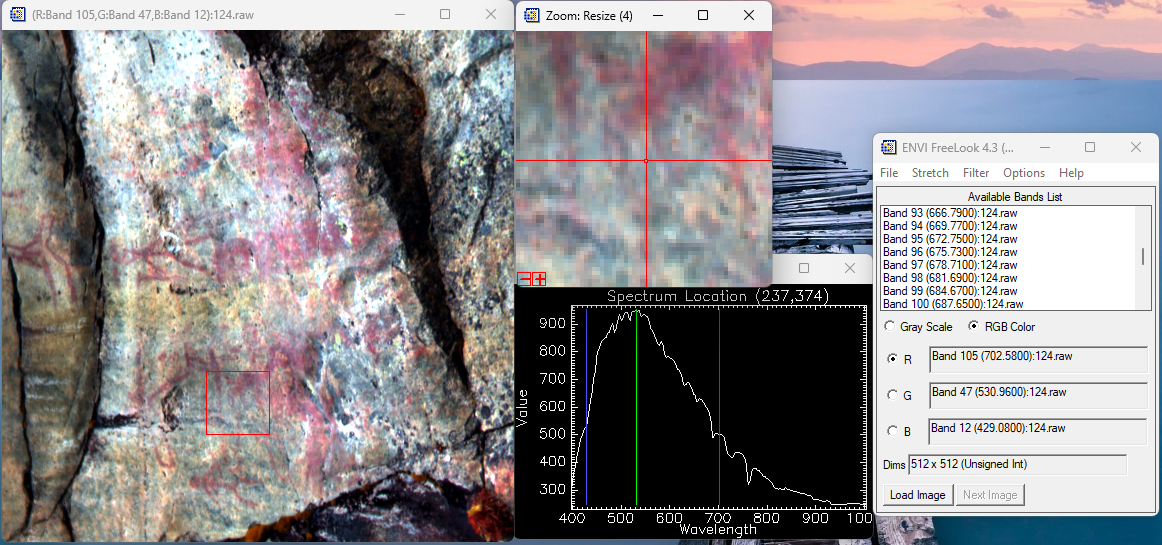
\includegraphics[width=0.45\textwidth]{figs/rock_painting_other.png}
    \label{fig:rock-painting-other}
  }
  \caption[]{RGB preview of rock paintings and spectra }
  \label{fig:rock-painting}
\end{figure}

\section{Tasks \#2. Study csv spectra of different materials}

